\usetikzlibrary{shapes,positioning,fit}
\usetikzlibrary{calc}	%for centerarc
\def\centerarc[#1](#2)(#3:#4:#5)% Syntax: [draw options] (center) (initial angle:final angle:radius)
{ \draw[#1] ($(#2)+({#5*cos(#3)},{#5*sin(#3)})$) arc (#3:#4:#5); }
\tikzset{
    container/.style={
        draw, rectangle, dashed, inner sep=0.75em
    }
}
\fontsize{1em}{1.1em}\selectfont
	%from Bergson - Matter and Memory, p. 211 (fig. 3)
	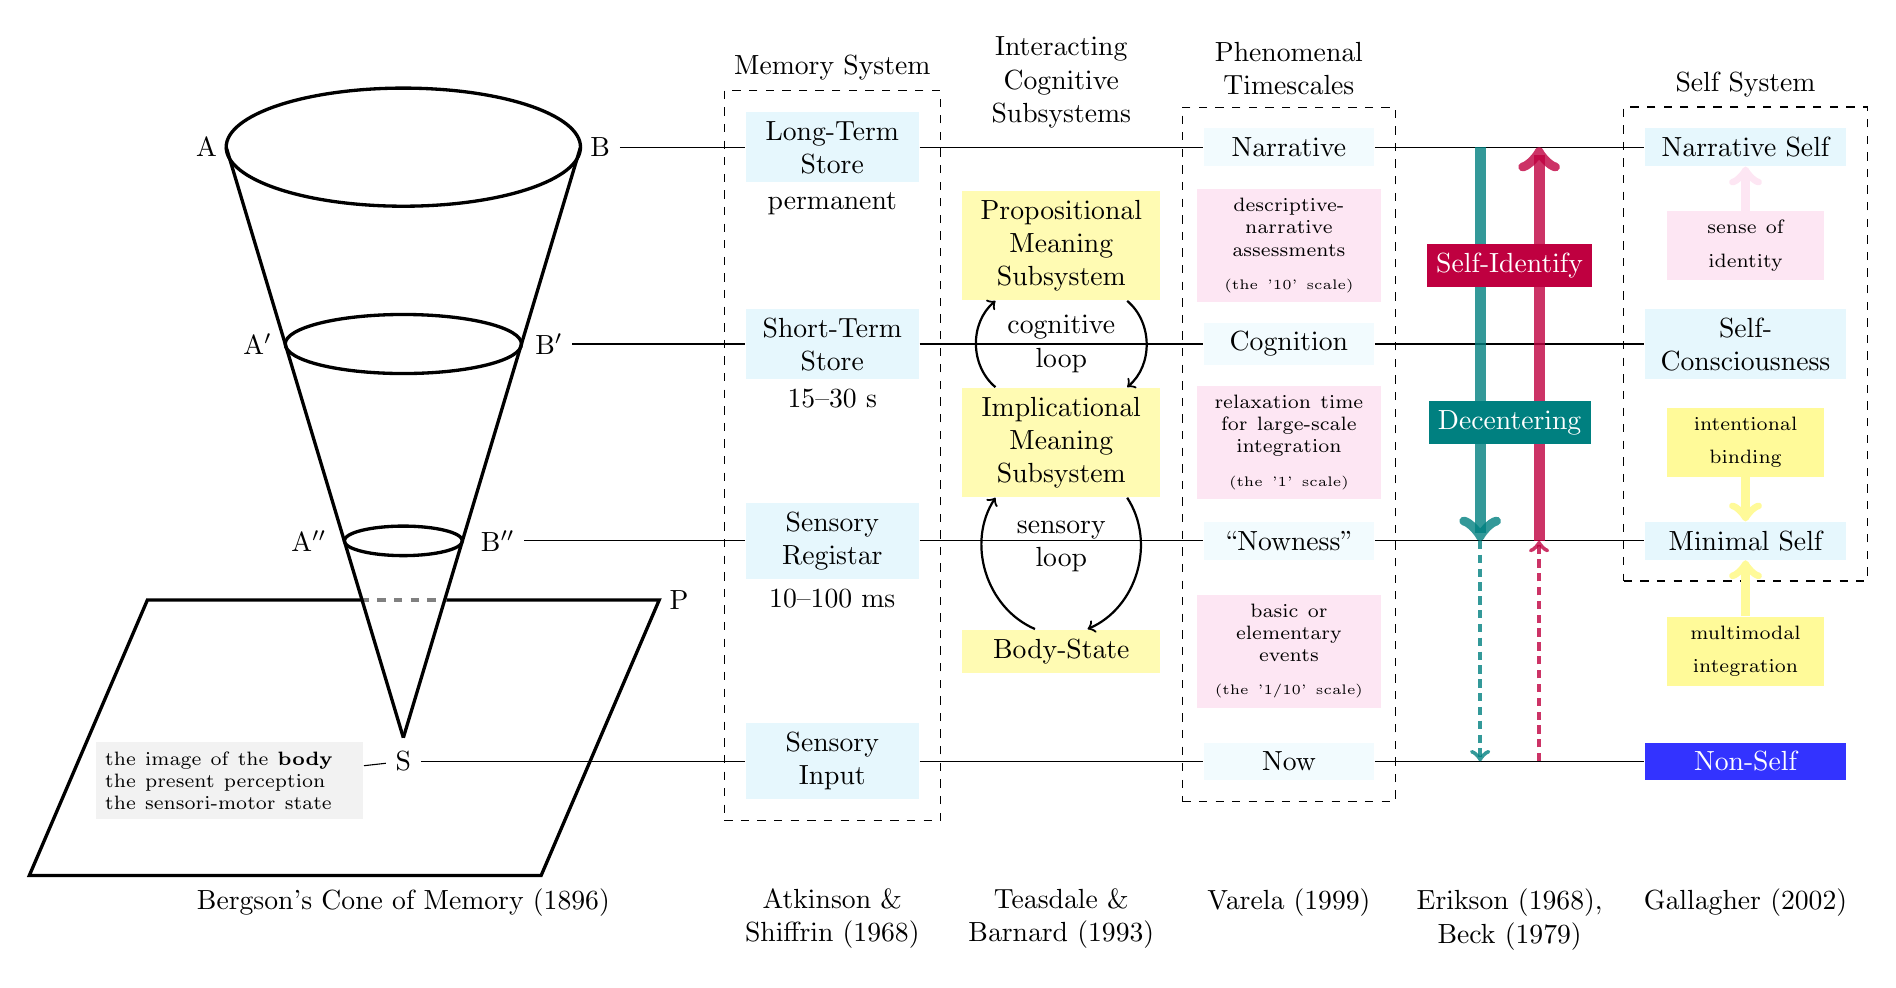
\begin{tikzpicture}[scale=1]
	%parallelogram
	\draw[very thick] (3.25,1.75)--(-3.25,1.75)--(-4.75,-1.75)--(1.75,-1.75)--cycle;
	\draw[ultra thick,white] (-0.54,1.75)--(0.55,1.75);
	\draw[very thick,dashed,gray] (-0.54,1.75)--(0.55,1.75);

	%triangle
	\draw[very thick] (0,0)--(-2.25,7.5);	%leftwards line
	\draw[very thick] (0,0)--( 2.25,7.5);	%rightward line
	
	%ellipses
	\draw[very thick] (0,7.5) ellipse (2.25cm and 0.75cm);
	\draw[very thick] (0,5.0) ellipse (1.5cm and 0.375cm);
	\draw[very thick] (0,2.5) ellipse (0.75cm and 0.1875cm);
	
	%labels
	\node (S) at (0,-0.3)	{S};
	\node at (3.5,1.75) {P};
	\node (A) at (-2.5,7.5) {A};	\node (Ap) at (-1.85,5)	{A$'$};		\node (App) at (-1.2,2.5) {A$''$};
	\node (B) at ( 2.5,7.5) {B};	\node (Bp)  at ( 1.85,5)	{B$'$};		\node (Bpp)  at ( 1.2,2.5) {B$''$};
	\node (V) at ( 0,7.5) {};	\node (Vp)  at (0,5)	{};		\node (Vpp)  at (0,2.5) {};
	\node[below=1.5 of S.center] {Bergson's Cone of Memory (1896)};

%%%%%%% modified %%%%%%%%

	\node[rectangle, fill=gray!10, text width=90, left=0.5 of S.south] (Body) {{\scriptsize the image of the $\mathbf{body}$ \\ the present perception\\ the sensori-motor state \par}}; %% \\ the present perception\\ the sensori-motor state
	\draw[thin] (S)--(Body);	%B to 


	%Sense

	\node[rectangle, fill=cyan!10, text width=56, text centered, right of=V, node distance=155] (LTM){Long-Term Store};
	\node[text width=56, text centered, below= 0 of LTM] (){permanent};
	\node[rectangle, fill=cyan!10, text width=56, text centered, right of=Vp, node distance=155] (STM){Short-Term Store};
	\node[text width=56, text centered, below= 0 of STM] (){15–30 s};
	\node[rectangle, fill=cyan!10, text width=56, text centered, right of=Vpp, node distance=155](SenM) {Sensory Registar};
	\node[text width=56, text centered, below= 0 of SenM] (Decay){10–100 ms };
	\node[rectangle, fill=cyan!10, text width=56, text centered, right of=S, node distance=155](Input)	{Sensory Input};
	\node[container, fit=(LTM) (Input)] (Msys) {};
	\node[above=0 of Msys] (MS) {Memory System};
	\node[below=1.5 of Input.center, text width=80, text centered] () {Atkinson \& Shiffrin (1968)};
	

	%edge to sense
	\draw[thin] (B)--(LTM);	%B to 
	\draw[thin] (Bp)--(STM);	%B' to 
	\draw[thin] (Bpp)--(SenM);	%B' to 
	\draw[thin] (S)--(Input);	%S to 

%%%%%%%

	%Varela's Time WIndow
	\node[rectangle, fill=cyan!5, text width=55, text centered, right of=LTM, node distance=165] (Narrative) 	{Narrative};
	\node[rectangle, fill=cyan!5, text width=55, text centered, right of=STM, node distance=165] (Cognition)		{Cognition};
	\node[rectangle, fill=cyan!5, text width=55, text centered, right of=SenM, node distance=165] (Nowness) 	{``Nowness''};
	\node[rectangle, fill=cyan!5, text width=55, text centered, right of=Input, node distance=165] (Now)		{Now};
	\node[rectangle, fill=magenta!10, text width=60, text centered] at ($(Narrative)!.5!(Cognition)$) (NT) {\scriptsize descriptive-narrative assessments \par \tiny (the '10' scale) };
	\node[rectangle, fill=magenta!10, text width=60, text centered] at ($(Nowness)!.5!(Cognition)$) {\scriptsize relaxation time for large-scale integration \par \tiny (the '1' scale) };
	\node[rectangle, fill=magenta!10, text width=60, text centered ]at ($(Now)!.5!(Nowness)$) (ET) {\scriptsize basic or elementary events \par \tiny (the '1/10' scale) };
	\node[container, fit=(Narrative) (Now)] (TS) {};
%	\node[above=0 of Ssys] {Self System};
	\node[text width=80, text centered, right of=MS, node distance=165] () {Phenomenal Timescales};
	\node[below=1.5 of Now.center, text width=80, text centered] {Varela (1999)};


	%edge to timescale
	\draw[thin] (LTM)--(Narrative) node[midway] (T1){};	%B to 
	\draw[thin] (STM)--(Cognition) node[midway] (T2){};	%B' to 
	\draw[thin] (SenM)--(Nowness) node[midway] (T3){};	%B' to 
	\draw[thin] (Input)--(Now) node[midway] (T4){};	%B' to 
%
%%%%%%%%%
%
	%ICS
	\node[rectangle, fill=yellow!30, text width=65, text centered] at ($(T1)!.5!(T2)$) (PS) {Propositional Meaning Subsystem};
	\node[rectangle, fill=yellow!30, text width=65, text centered] at ($(T2)!.5!(T3)$) 	(IS)  {Implicational Meaning Subsystem};
	\node[rectangle, fill=yellow!30, text width=65, text centered] at ($(T3)!.5!(T4)$)	(BS) {Body-State};
	\node[text width=65, text centered, above=0.00 of T1] {Interacting Cognitive Subsystems};
	\node[text width=75, text centered, below=1.5 of T4.center] {Teasdale \& Barnard (1993)};

	\draw [->,thick] (PS) to [bend left=50] node[below] {} (IS);
	\draw [->,thick] (IS) to [bend left=50] node[below] {} (PS);
	\node[rectangle, text width=50, text centered] at ($(IS)!.5!(PS)$) {cognitive loop};
	\draw [->,thick] (IS) to [bend left=50] node[below] {} (BS);
	\draw [->,thick] (BS) to [bend left=50] node[below] {} (IS);
	\node[rectangle, text width=50, text centered] at ($(BS)!.5!(IS)$) {sensory loop};
%
%
%
%
%
%
%
	%Self
	\node[rectangle, fill=cyan!10, text width=66, text centered, right of=Narrative, node distance=165] (Nself) 	{Narrative Self};
	\node[rectangle, fill=cyan!10, text width=66, text centered, right of=Cognition, node distance=165] (Sawa)		{Self-Consciousness};
	\node[rectangle, fill=cyan!10, text width=66, text centered, right of=Nowness, node distance=165] (Mself) 	{Minimal Self};
	\node[rectangle, fill=blue!80, text width=66, text centered, right of=Now, node distance=165,text=white] (Non)		{Non-Self};
	\node[container, fit=(Nself) (Mself)] (Ssys) {};
	\node[above=0 of Ssys] {Self System};
	\node[rectangle, fill=magenta!10, text width=50, text centered] at ($(Sawa)!.5!(Nself)$) (SI) {\scriptsize sense of identity };
	\draw[->,ultra thick,opacity=1.0,magenta!10,line width=3]  (SI)--(Nself) node [midway] () {};
	\node[rectangle, fill=yellow!40, text width=50, text centered] at ($(Sawa)!.5!(Mself)$) (IB) {\scriptsize intentional binding };
	\draw[->,ultra thick,opacity=1.0,yellow!40,line width=3]  (IB)--(Mself) node [midway] () {};
	\node[rectangle, fill=yellow!40, text width=50, text centered] at ($(Mself)!.5!(Non)$) (MI) {\scriptsize multimodal integration };
	\draw[->,ultra thick,opacity=1.0,yellow!40,line width=3]  (MI)--(Mself) node [midway] () {};
	\node[below=1.5 of Non.center, text width=80, text centered] {Gallagher (2002)};
%
	%edge to self
	\draw[thin] (Narrative)--(Nself) node[midway] (E1){};	%B to 
	\draw[thin] (Cognition)--(Sawa) node[midway] (E2){};	%B' to 
	\draw[thin] (Nowness)--(Mself) node[midway] (E3){};	%B' to 
	\draw[thin] (Now)--(Non) node[midway] (E4){};	%B' to 
	\node[below=1.5 of E4.center, text width=80, text centered] {Erikson (1968), Beck (1979)};

	%Decentering/Identify
	\coordinate[left=0.25 of E1] (P2);
	\coordinate[left=0.25 of E3] (P1);
	\coordinate[left=0.25 of E4] (P0);
	\coordinate[right=0.25 of E1]  (P4){};
	\coordinate[right=0.25 of E3]  (P3){};
	\coordinate[right=0.25 of E4]  (P02){};
	\draw[->,ultra thick,opacity=.8,teal,line width=4]  (P2)--(P1) node [midway] (P5) {};
	\draw[->,ultra thick,opacity=.8,teal,densely dashed]  (P1)--(P0) node [midway]  {};
	\draw[<-,ultra thick,opacity=.8,purple,line width=4]  (P4)--(P3) node [midway] (P6) {};
	\draw[->,ultra thick,opacity=.8,purple,densely dashed]  (P02)--(P3) node [midway]  {};
	\node [rectangle, fill=teal,text=white]  at ($(E1)!0.5!(E3)+(0,-1)$) {Decentering};
	\node [rectangle, fill=purple,text=white]  at ($(E1)!0.5!(E3)+(0,1)$) {Self-Identify};


	\end{tikzpicture}